\chapter{等额年金}
\begin{introduction}
	\item 每年支付m次的年金
	\item 连续支付的等额年金
\end{introduction}
\section{符号一览}
\noindent$a_{\angles{n}},s_{\angles{n}}$\\	$\ddot{a}_{\angles{n}}$\\$\ddot{s}_{\angles{n}}$
\section{等额年金}
\begin{definition}{年金的终值与现值}
\noindent $a_{\angles{n}},s_{\angles{n}}$\\
$s_{\angles{n}}=a_{\angles{n}}(1+i)^{n}=\frac{(1+i)^{n}-1}{i}$
\end{definition}
\begin{definition}{Accumulated Value of an $n$ -Payment Annuity-Immediate of 1 Per Period}

	The symbol $s_{\angles{n}}$ denotes the accumulated value, at the time of (and including) the final payment of a series of $n$ payments of 1 each made at equally spaced intervals of time, where the rate of interest per payment period is $i$
	$\begin{aligned}
	s_{\angles{n}} &=(1+i)^{n-1}+(1+i)^{n-2}+\cdots+(1+i)+1 \\
	&=\sum_{t=0}^{n-1}(1+i)^{t}=\frac{(1+i)^{n}-1}{i}
	\end{aligned}$
\end{definition}
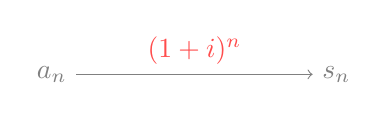
\begin{tikzpicture}
\draw [color=black!50,->](0,0) node[left]{$a_{\angles{n}}$}-- node [color=red!70,pos=0.5,above,sloped]{$(1+i)^n$}(3,0) node[right]{$s_{\angles{n}}$};
    \end{tikzpicture} \\
\noindent $a_{\angles{n}}=v+v^2+v^3+\dots+v^n=\frac{1-v^n}{i}=\frac{1-\frac{1}{(1+i)^n}}{i}=\frac{1-v^n}{\frac{1}{v}-1}$\\
\begin{lstlisting}[language={python}]
#wolframalpha
(1-(1/(1+i)^n))/i=(1-v^n)/(1/v-1)
\end{lstlisting}
$\ddot{a}_{\angles{n}}=\frac{1-v^n}{d}$ \\
$s_{\angles{n}}=a_{\angles{n}}(1+i)^{n}=\frac{(1+i)^{n}-1}{i}$\\
$\ddot{s}_{\angles{n}}=\ddot{a}_{\angles{n}}(1+i)^{n}=\frac{(1+i)^{n}-1}{d}$
\begin{property}
$1=i{a}_{\angles{n}}+v^n$
\end{property}
 \begin{definition}{每年支付m次年金}
 \noindent ${a}_{\angles{n}}^{\(m\)}=\frac{1-v^n}{i^{(m)}}$ 
 \end{definition}
 